%!TEX root = ../main.tex
\section{Introduction} 
\label{sec:intro}
Introduction here.

\stitle{Problem.}
Our main research question in this paper is how to \textit{detect mislabeled data in the large training set which will be used for the downstream meachine learning model} and filter it to improve the data quality of training set.

A positive answer to this question is crucial as it can help machine learning model to learn more correctly about the distribution of the training set, so as to obtain better model performance.


\stitle{Challenges.}
\nan{Add after we have the technical sections.}


\stitle{Our Proposal.}
Our main idea is to find out the instance in the training set which is labeled incorrectly.
More specifically, \nan{Add more details later.}

\stitle{Contributions.}
Our contributions are summarized as follows:

\be
	\item 
	\item 
	\item \nan{If we can have a good summary of experiments, we can either add here or use a ``stitle'' section to highlight the empirical findings.}
\ee


% \begin{figure*}
%	\centering
%	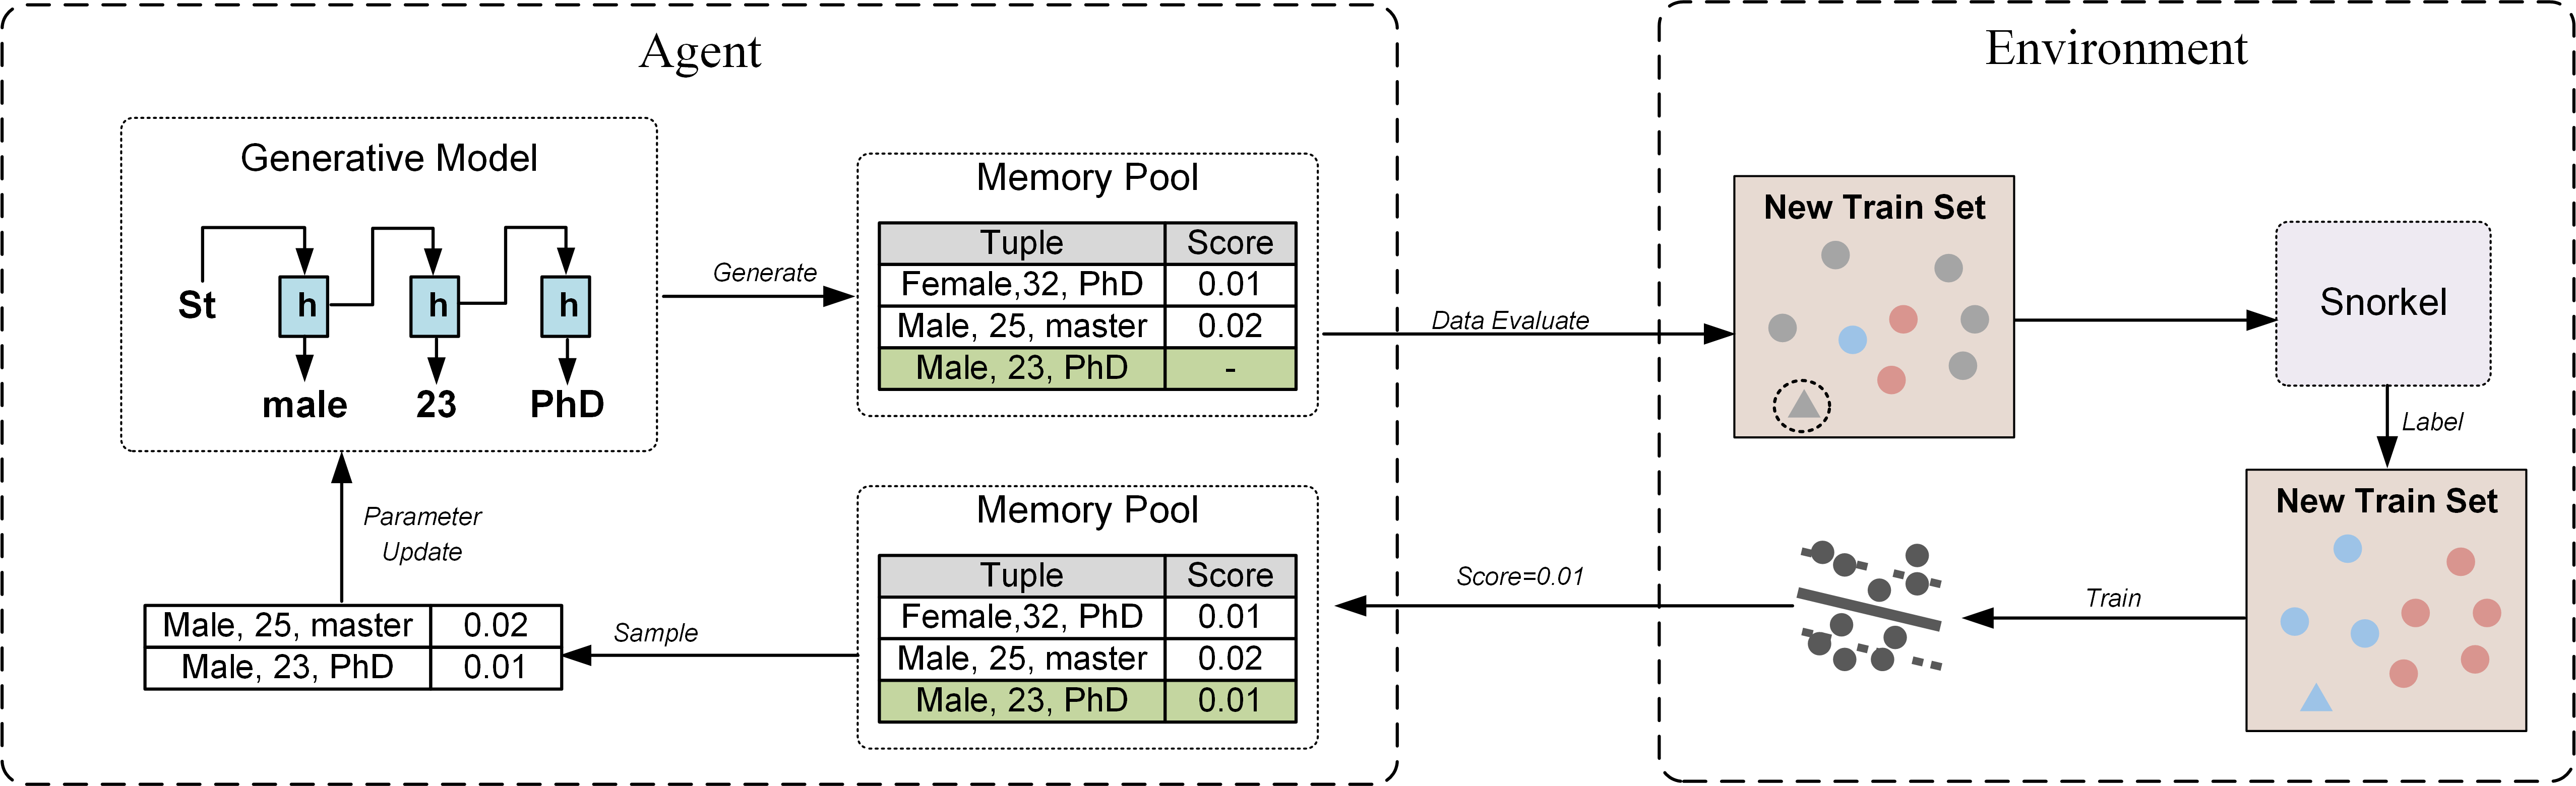
\includegraphics[width=\textwidth]{figures/overview.png}
%	\caption{Framework}
%	\label{fig:framework}
% \end{figure*}

% \begin{itemize}
% 	\item The difference between traditional data generation and ours (for ML model).
% 	\item (Challenge) The key challenges of this problem: learn the generative model from feedback; how to evaluate generated tuples.
% \end{itemize}